\documentclass[handout]{beamer}\mode<presentation>{\usetheme{AMSCesenaBleu}}

\usepackage{multicol}
\usepackage{common}
\usepackage{pgfpages}
\usepackage{subfigure}
\usepackage{media9}
\usepackage{xargs} % Use more than one optional parameter in a new commands % Coloured text etc.
\usepackage[colorinlistoftodos,prependcaption]{todonotes}

\newcommandx{\unsure}[2][1=]{\todo[linecolor=red,backgroundcolor=red!25,bordercolor=red,#1]{#2}}
\newcommandx{\change}[2][1=]{\todo[linecolor=blue,backgroundcolor=blue!25,bordercolor=blue,#1]{#2}}
\newcommandx{\improvement}[2][1=]{\todo[linecolor=ForestGreen,backgroundcolor=ForestGreen!25,bordercolor=ForestGreen,#1]{#2}}
\newcommandx{\marianiSays}[2][1=]{\todo[linecolor=Orange,backgroundcolor=Orange!25,bordercolor=Orange,#1]{#2}}

%\setbeameroption{show notes on second screen=right}

% \graphicspath{{res/img/}}

%\AtBeginSection[]
%{
%\begin{frame}<beamer>[c]\frametitle{A seguire\ldots}
%		\tableofcontents[currentsection,hideallsubsections]
%\end{frame}
%}

\newenvironment{nscenter}
{\parskip=1pt\par\nopagebreak\centering}
{\par\noindent\ignorespacesafterend}

\title[Prolog BDI agents on Alchemist]{Simulazione di agenti BDI basati su Prolog in Alchemist}
\author[Filippo Nicolini]{Tesi in: Sistemi Autonomi\\
[0.5cm]
\textit{Relatore:} \hspace{6.55cm} \textit{Presentata da:}\\
Chiar.mo Prof. \hspace{5.5cm} Filippo Nicolini\\
Andrea Omicini \hspace{7.6cm} \phantom{g}\\
\textit{\\Correlatori:} \hspace{8.25cm} \phantom{g}\\
Dott. Ing. Danilo Pianini \hspace{6cm} \phantom{g}\\
Dott. Giovanni Ciatto \hspace{6.5cm} \phantom{g}\\
}
\institute[]{
\textsc{Alma Mater Studiorum} -- Università di Bologna \\
Campus di Cesena}
\date{12 Dicembre 2019}

\begin{document}

\maketitle


\section{Introduzione}

\subsection{Obiettivo}
%Slide 1
\begin{frame}
\frametitle{L'obiettivo della tesi}
\begin{block}{Obiettivo della tesi}
\alert{Unificare} piattaforme orientate alla \alert{programmazione di agenti} con ambienti di \alert{simulazione di agenti}.
\end{block}

\begin{block}{Interprete tuProlog}
Estensione modello BDI di AgentSpeak sfruttando tuProlog per poter implementare interpreti sia su ambienti reali che simulati.
\end{block}

\begin{block}{Interprete Alchemist}
Realizzazione di un interprete nel simulatore Alchemist che utilizza le logiche del ciclo di ragionamento di Jason.
\end{block}
\end{frame}


\section{Struttura agente}

\subsection{Stato dell'arte}

%Slide 2
\begin{frame}
\frametitle{AgentSpeak e modello BDI}
\begin{block}{Modello BDI}
Modello BDI (Beliefs, Desires, Intentions) implementa gli aspetti principali del ragionamento umano per programmare agenti intelligenti.
\end{block}
\begin{block}{AgentSpeak}
Linguaggio orientato agli agenti basato su modello BDI e programmazione logica.
\end{block}
\end{frame}

%Slide 3
\begin{frame}
\frametitle{tuProlog}
\begin{block}{tuProlog}
Libreria che permette di utilizzare Prolog all'interno di applicazioni e infrastrutture distribuite sfruttando un core minimale.
\end{block}

\begin{block}{Caratteristiche}
Supporta integrazioni semplice e pervasiva multi-linguaggio e multi-paradigma (es. Prolog -- linguaggi OO).

\end{block}
\end{frame}


\subsection{Interprete Prolog}

%Slide 4
\begin{frame}
\frametitle{Interprete tuProlog di AgentSpeak}
\begin{block}{Formalizzazione}
Estenzione di AgentSpeak realizzando un'interprete attraverso definizione di alcune sintassi.
\end{block}

\begin{block}{API}
\begin{itemize}
\item inizializzazione agente
\item invocazioni verso linguaggio OO
\item gestione `belief base'
\item gestione eventi e posizionamento
\end{itemize}
\end{block}
\end{frame}



\section{Comportamento agente}

\subsection{Stato dell'arte}

%Slide 5
\begin{frame}
\frametitle{Alchemist}
\begin{block}{Alchemist}
Simulatore per il calcolo pervasivo, aggregato e naturale che si basa su un meta-modello flessibile e che permette implementazioni di modelli diversi tra loro.
\end{block}
\begin{block}{Meta-modello}
\begin{itemize}
\item Node
\item Environment
\item Reaction (Time Distribution, Condition, Action)
\item Linking Rule
\end{itemize}
\end{block}
\end{frame}

%Slide 6
\begin{frame}
\frametitle{Meta-modello}
\begin{figure}
\includegraphics[width=9cm]{images/alchemistModel.png}
\end{figure}
\end{frame}

%Slide 7
\begin{frame}
\frametitle{Spazi di tuple}
\begin{block}{LINDA}
Modello di coordinazione e comunicazione tra processi paralleli con memoria associativa, virtuale, condivisa.
\end{block}
\begin{block}{Spatial Tuples}
Estensione del modello base di tuple per i sistemi distribuiti multi-agente.
\vspace{0.2cm}

Operazioni consentite
\begin{itemize}
\item in: legge tupla e la consuma
\item rd: legge tupla senza consumarla
\item out: inserisce tupla
\end{itemize}
\end{block}
\end{frame}

\subsection{Interprete Alchemist}

%Slide 8
\begin{frame}
\frametitle{Ciclo di ragionamento}
\begin{block}{Percezioni}
Informazioni ricevute tramite un apparato con le quali l'agente percepisce i cambiamenti dell'ambiente.
\end{block}

\begin{block}{Eventi}
Sono relativi a percezioni che l'agente ha ricevuto e possono essere catturati dall'agente.
\end{block}

\begin{block}{Piani}
Definiscono come l'agente agisce per raggiungere goal.
\end{block}

\begin{block}{Intenzioni}
Operazioni che l'agente vuole eseguire per portare a termine un certo goal.
\end{block}
\end{frame}

%Slide 9
\begin{frame}
\frametitle{Ciclo di ragionamento}
\begin{figure}
\hspace*{-0.35cm}
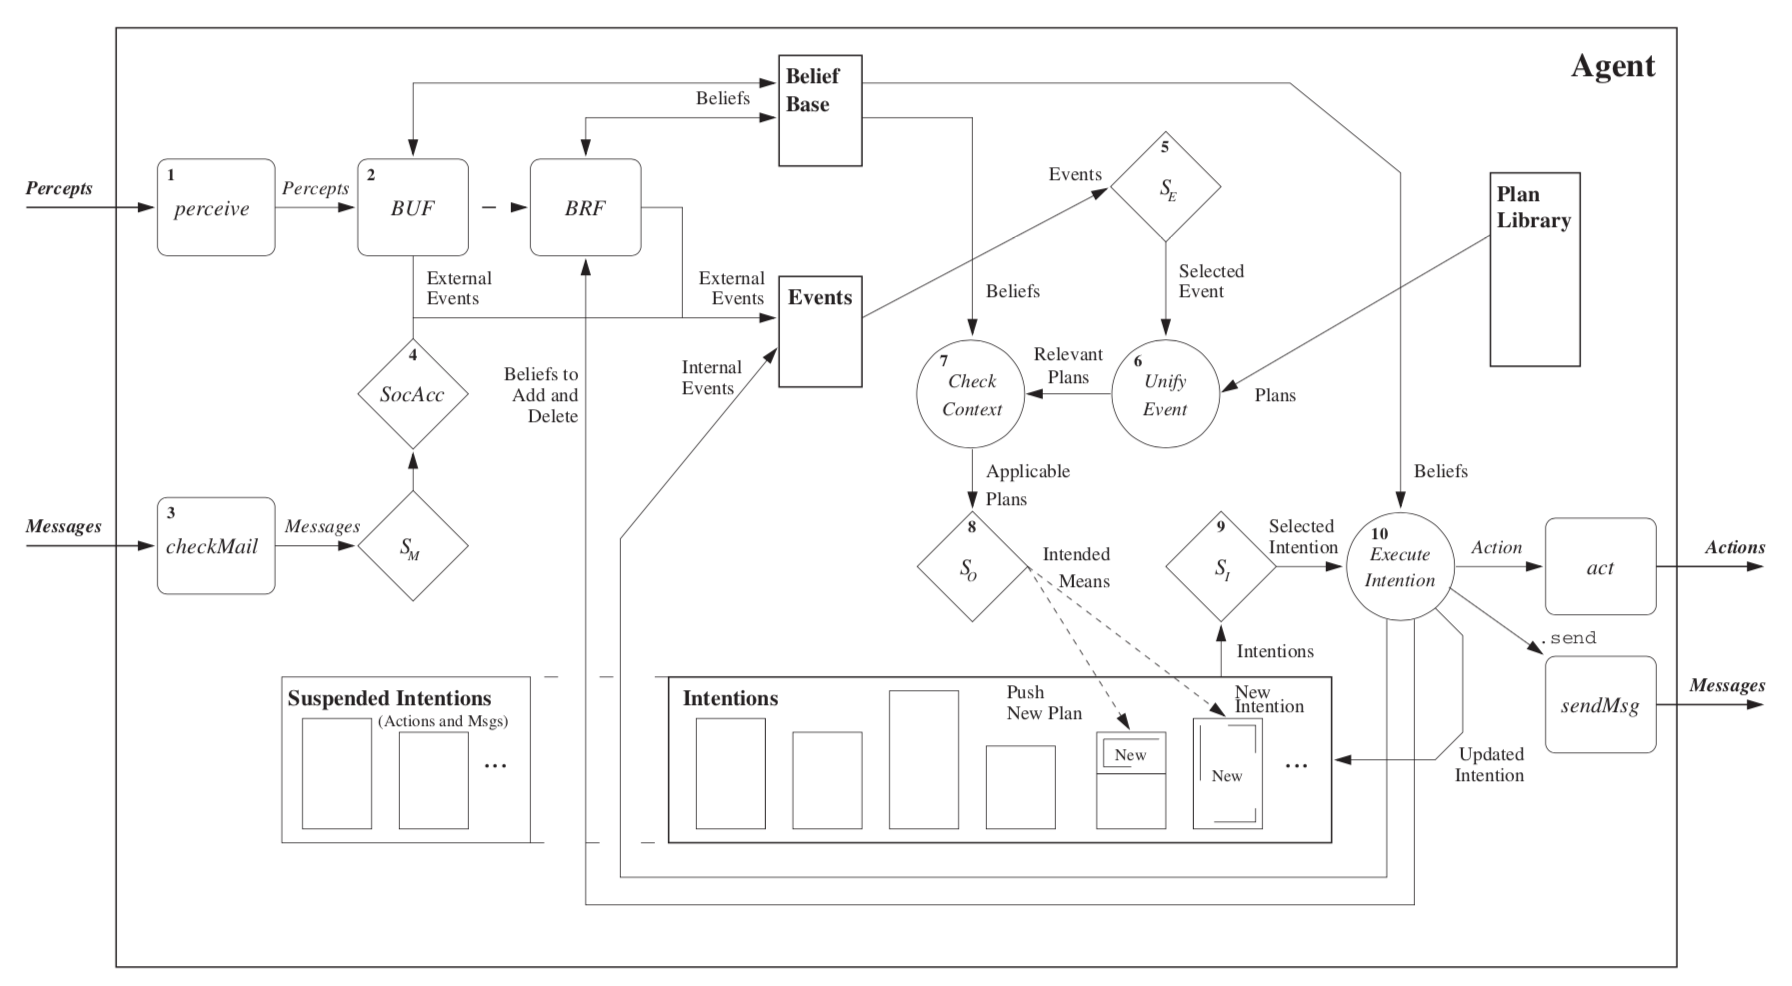
\includegraphics[width=12.5cm]{images/reasoningCicle.png}
\end{figure}
\end{frame}

%Slide 10
\begin{frame}
\frametitle{Unione modelli}
\begin{block}{Mapping}
\begin{center}
\alert{Environment} $\rightarrow$ Spazio agenti \hspace{1.5cm} \alert{Nodo} $\rightarrow$ Contenitore agenti \\
\alert{Reazione} $\rightarrow$ Agente
\end{center}
\end{block}
\begin{figure}
\includegraphics[width=7cm]{images/alchemistReaction.png}
\end{figure}

\begin{block}{Caratteristiche mapping}
Ricercata la massima espressività lavorando su più strati: nodo può essere inteso come device in cui operano più agenti.
\end{block}




%\begin{block}{Mapping}
%%Agente mappato come reazione, quindi l'ambiente è contenitore di nodi che a loro volta contengono uno o più agenti.
%\begin{center}
%\begin{tabular}{ | c || c | c | }
%\hline
% Alchemist\textbackslash  AgentSpeak & Agente & Ambiente \\\hline\hline
% Reazione & cell5 & cell6 \\\hline
% Nodo & cell8 & cell9 \\\hline
%\end{tabular}
%\end{center}
%\end{block}
\end{frame}



\section{Caso di studio}
\subsection{Scenario}
%Slide 11
\begin{frame}
\frametitle{Scenario}
\begin{block}{Goldminers}
Un gruppo di minatori deve recuperare pepite d'oro da miniere sparse nell'ambiente e riportarle in un deposito.
\end{block}
\begin{block}{Entità $\rightarrow$ ruoli}
All'interno del problema si individuano le seguenti entità:
\begin{itemize}
\item \alert{minatori} $\rightarrow$ \alert{agenti}
\item pepite $\rightarrow$ tuple
\item \alert{miniere} $\rightarrow$ \alert{spazi di tuple}
\item deposito $\rightarrow$ agente
\end{itemize}
\end{block}
\end{frame}

\begin{frame}
\frametitle{Realizzazione}
\begin{block}{Minatore}
Comportamento diviso in 4 stati:
\begin{itemize}
\item \alert{ricerca}: spostamento casuale emettendo richieste di tuple;
\item \alert{ricezione tupla}: salva posizione miniera e si dirige al deposito;
\item \alert{arrivo deposito}: invio pepita e si dirige posizione miniera salvata;
\item \alert{arrivo miniera}: torna stato ricerca. 
\end{itemize}
\end{block}
\begin{block}{Miniera}
Istanzia N tuple all'inizializzazione e risponde alle richieste dei minatori.
\end{block}
\begin{block}{Deposito}
Statico nell'ambiente, riceve la pepita tramite un messaggio.
\end{block}
\end{frame}

\section{Conclusioni}
\begin{frame}
\frametitle{Conclusioni e lavori futuri}
\begin{block}{Conclusioni}
\begin{itemize}
\item Realizzazione di interprete per programmare e simulare agenti
\item Forte espressività modello e interprete (Prolog e OO)
\item Estensione agenti in spazi di tuple 
\end{itemize}
\end{block}
\begin{block}{Lavori futuri}
\begin{itemize}
\item Implementazione interprete OO in piattaforme per ambiente reale
\item Ricerca per migliorie sia nell'interprete Prolog che nell'interprete OO
\end{itemize}
\end{block}
\end{frame}

\section{}
\subsection{}
\maketitle

\end{document}
